\usetikzlibrary{fit}

\definecolor{blue}{rgb}{0.9,0.96,1}
\definecolor{beige}{rgb}{1,0.96,0.90}
\definecolor{green}{rgb}{0.96,1,0.96}

\tikzstyle{label} = [align=center]
\tikzstyle{node_init} = [align=center, fill=blue, rectangle, minimum width=2cm, minimum height=1cm, text centered, draw=black]
\tikzstyle{node_improv} = [align=center, fill=beige, rectangle, minimum width=2cm, minimum height=1cm, text centered, draw=black]
\tikzstyle{node_final} = [align=center, fill=green, rectangle, minimum width=2cm, minimum height=1cm, text centered, draw=black]
\tikzstyle{init} = [rectangle, rounded corners, minimum width=3cm, minimum height=3.8cm, text centered, draw=black]
\tikzstyle{improvement} = [rectangle, rounded corners, minimum width=7cm, minimum height=3.8cm, text centered, draw=black]
\tikzstyle{arrow} = [->,>=stealth]

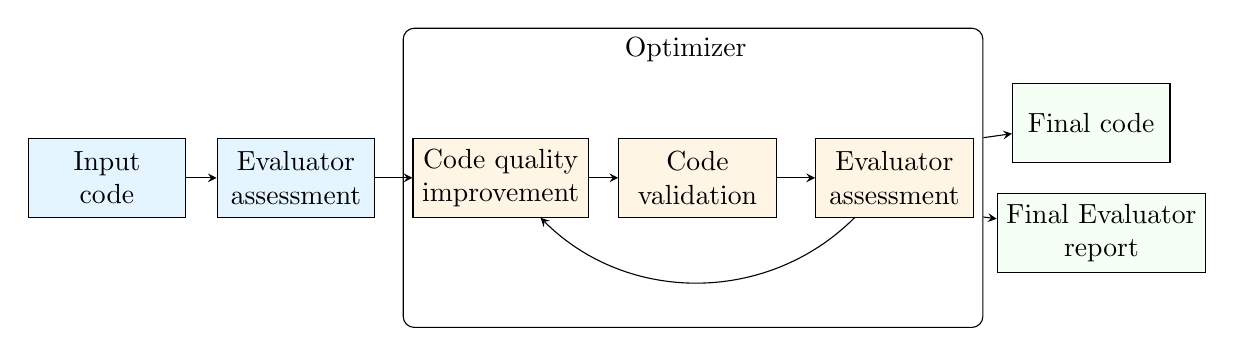
\begin{tikzpicture}[node distance=2cm]

\node (node0) [node_init] {Input\\code};
\node (node1) [node_init, xshift=2.4cm] {Evaluator\\assessment};
\node (node2) [node_improv, xshift=5cm] {Code quality\\improvement};
\node (node3) [node_improv, xshift=7.5cm] {Code\\validation};
\node (node4) [node_improv, xshift=10cm] {Evaluator\\assessment};
\node (node5) [node_final, xshift=12.5cm, yshift=0.7cm] {Final code};
\node (node6) [node_final, xshift=12.63cm, yshift=-0.7cm] {Final Evaluator\\ report};

% \node (init) [init, fit={(node0) (node1)}] {};
% \node (label_init) [label, yshift=1.63cm, xshift=1.35cm] {Initial Evaluation};
\node (improvement) [improvement, fit={(node2) (node3) (node4)}] {};
\node (label_improvement) [label, yshift=1.63cm, xshift=7.35cm] { Optimizer};

\draw [arrow] (node0) -- (node1);
\draw [arrow] (node1) -- (node2);
\draw [arrow] (node2) -- (node3);
\draw [arrow] (node3) -- (node4);
\draw [arrow] (improvement) -- (node5);
\draw [arrow] (improvement) -- (node6);

% Add curved arrows with labels
\draw [arrow, bend left=45] (node4) to (node2);
%\draw [arrow, bend left=45] (node2) to node[midway, above] {} (node4);
\end{tikzpicture}